%%% Local Variables:
%%% mode: latex
%%% TeX-master: "../cheat-sheet"
%%% End:

\begin{figure}[H]
  \centering
  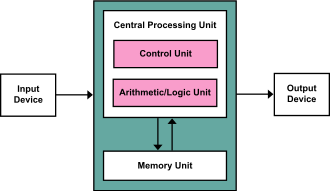
\includegraphics[width=8.0cm]{images/330px-Von_Neumann_Architecture.png}
  \caption{Von Neumann Architecture}
\end{figure}

\subsection{Processor}
There are different kinds of processors, the most widely used are
\begin{itemize}
	\item General purpose central processing units (CPUs, used in PCs)
	\item ASIC (application-specific integrated circuit)
	\item GPU (graphics processing units)
\end{itemize}

Operates in \textbf{cycles} (see~\nameref{sec:cpu-func} for details):
\begin{itemize}
	\item Fetch instruction (using the PC/IP)
	\item Decode instruction (there are different \emph{addressing modes})
	\item Execute - Control Unit and ALU (Arithmetic/Logic Unit)
\end{itemize}
(This is the so-called three-stage pipeline. There is also the modern superscalar CPU (see page 21 in DJ Tanenbaum's book))

\textbf{Word size} - Modern PCs use a word-size of 64 bits. Embedded systems using microcontrollers often have a smaller word size (modern ones have down to 8 bit)

\subsection{Register}
A processor register is a small amount of storage available as part of a digital processor, such as a CPU. Such registers are (typically) addressed by mechanisms other than main memory and can be accessed faster.


\begin{figure}[H]
  \centering
  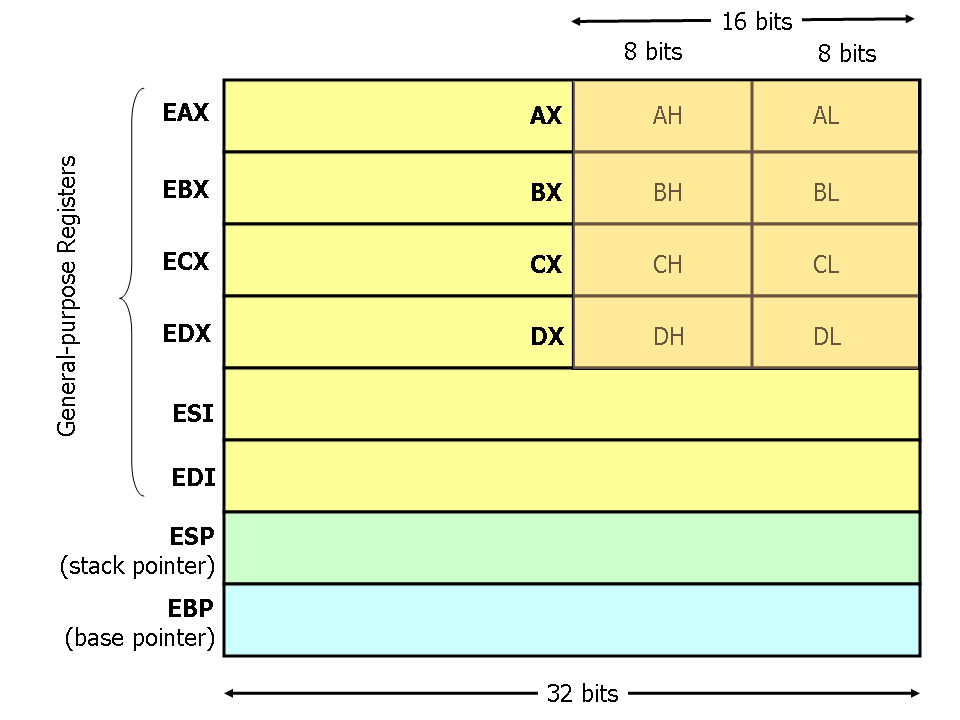
\includegraphics[width=8.0cm]{images/x86-registers}
  \caption{An overview of the registers (x86): }
\end{figure}

\subsection{Program counter / instruction pointer (PC/IP)}
A processor register that indicates where a computer is in its program sequence.

\subsection{Cache}
A CPU cache is used to reduce the average time to access data from the main memory. The cache is a smaller, faster memory which stores copies of the data from frequently used main memory locations.

In modern CPU's there are typically two \emph{layers of caches}, \textbf{L1} and \textbf{L2}. L1 cache is inside the CPU and feeds decoded instructions into the CPU's execution process. L2 cache holds several megabytes of recently used memory words. It is slower than L1, due to its size. Accessing L1 takes 1 cycle and acessing L2 takes 1 or 2 cycles.

On multicore chips, the placement of the L2 cache can vary. A single L2 cache can be shared by all the cores (intel).  This requires a more complicated cache controller. Another design is to give every core its own L2 cache (AMD). This is difficult to keep consistent.

\subsubsection{Cache cohorence}
A protocol for managing the caches of a multiprocessor system so that no data is lost or overwritten before the data is transferred from a cache to the target memory.

When multiple processors with separate caches share a common memory, it is necessary to keep the caches in a state of coherence by ensuring that any shared operand that is changed in any cache is changed throughout the entire system. This is done in either of two ways~\footnote{\url{http://www.webopedia.com/TERM/C/cache_coherence.html}}; through a directory-based or a snooping system:
\begin{enumerate}
\item In a directory-based system, the data being shared is placed in a common directory that maintains the coherence between caches. The directory acts as a filter through which the processor must ask permission to load an entry from the primary memory to its cache. When an entry is changed the directory either updates or invalidates the other caches with that entry.
\item In a snooping system, all caches on the bus monitor (or snoop) the bus to determine if they have a copy of the block of data that is requested on the bus. Every cache has a copy of the sharing status of every block of physical memory it has.
\end{enumerate}
Cache misses and memory traffic due to shared data blocks limit the performance of parallel computing in multiprocessor computers or systems. Cache coherence aims to solve the problems associated with sharing data.

\subsection{I/O device}
TODO

\subsection{Instruction set architecture (ISA)}
Well-defined software/hardware interface.

\begin{itemize}
	\item Functional definition - Operations and storage locations supported by hardware. With Intel's Ivy Bridge chip-architecture came the operation RdRand for instance, which is an operation that returns a hardware-generated random number.
	\item Documentation of how to use the instructions (see ABI below?).
\end{itemize}

(TODO: application binary interface (ABI). I believe this is contained within ISA. This defines the calling conventions for the architecture - for instance how system calls are carried out)
